% Comment with the percent symbol and use backslash (\) for commands in LaTeX
% Get signed up for Overleaf w/ VT email (if already have, add VT email for premium, although do not need for this workshop)
% Will lose access to premium once leave VT
% This is a new Blank Project in Overleaf, also check out the Example Project for more examples

% Add your author/update information in comments too towards the top - good practice for any code!:
% Author: Sarah Over, PhD - Virginia Tech
% Created: Feb 15, 2023
% Last Updated: Feb 17, 2023

\documentclass{article}  % What kind of document we are creating
\usepackage{graphicx} % Required for inserting images

% Packages added during workshop for additional features
\usepackage[colorlinks=true, linkcolor=blue, citecolor=blue, urlcolor=blue]{hyperref}  % Not used until end to create hyperlinks, but as it changes the appearance of cross references too, make sure to use optional commands
\usepackage{amsmath}  % For most math symbols and characters

\title{Beginners' Workshop}
\author{Sarah Over, PhD}
\date{February 2023}



\begin{document}  % after this the content starts (above is the preamble/setup)

\maketitle  % tells LaTeX we want our title here


\section{Introduction} % Just need to use the section command and LaTeX automatically numbers it (and index it for a table of contents - not added in this example)

Here is my first sentence in \LaTeX!
Here is (not) a new paragraph. % did not show on new line - need line in between for it to be a new paragraph

To edit text look you can use \tiny for tiny text \normalsize and \huge for huge text. \normalsize Just remember to go back to normal text! % See https://www.overleaf.com/learn/latex/Font_sizes%2C_families%2C_and_styles for more info on font sizing

You can also use \textbf{for bold} and \textit{or} \emph{for italics}. For special text characters use \`e or similar depending on the character.

To add website links and other hyperlinked objects, use the \href{https://ctan.org/pkg/hyperref}{hyperref package}.


\section{Floats} % See the placeins package to place float barriers to keep them close to text

\subsection{Figures} % Can also do subsections (and subsubsections for organization)
You can add figures with a begin command:

% Can upload directly or enter a web address for figures as was done in the workshop.  This is a big figure - need to set scale, but textwidth command convenient (try taking away the part in brackets with the textwidth command).  If your figure(s) slow things down, try compiling in draft mode using (select using arrow down to right of "Recompile").
\begin{figure}[h]  % [] are used for optional parts of commands, 'h' means here - if it cannot go here, LaTeX will warn
    \centering
    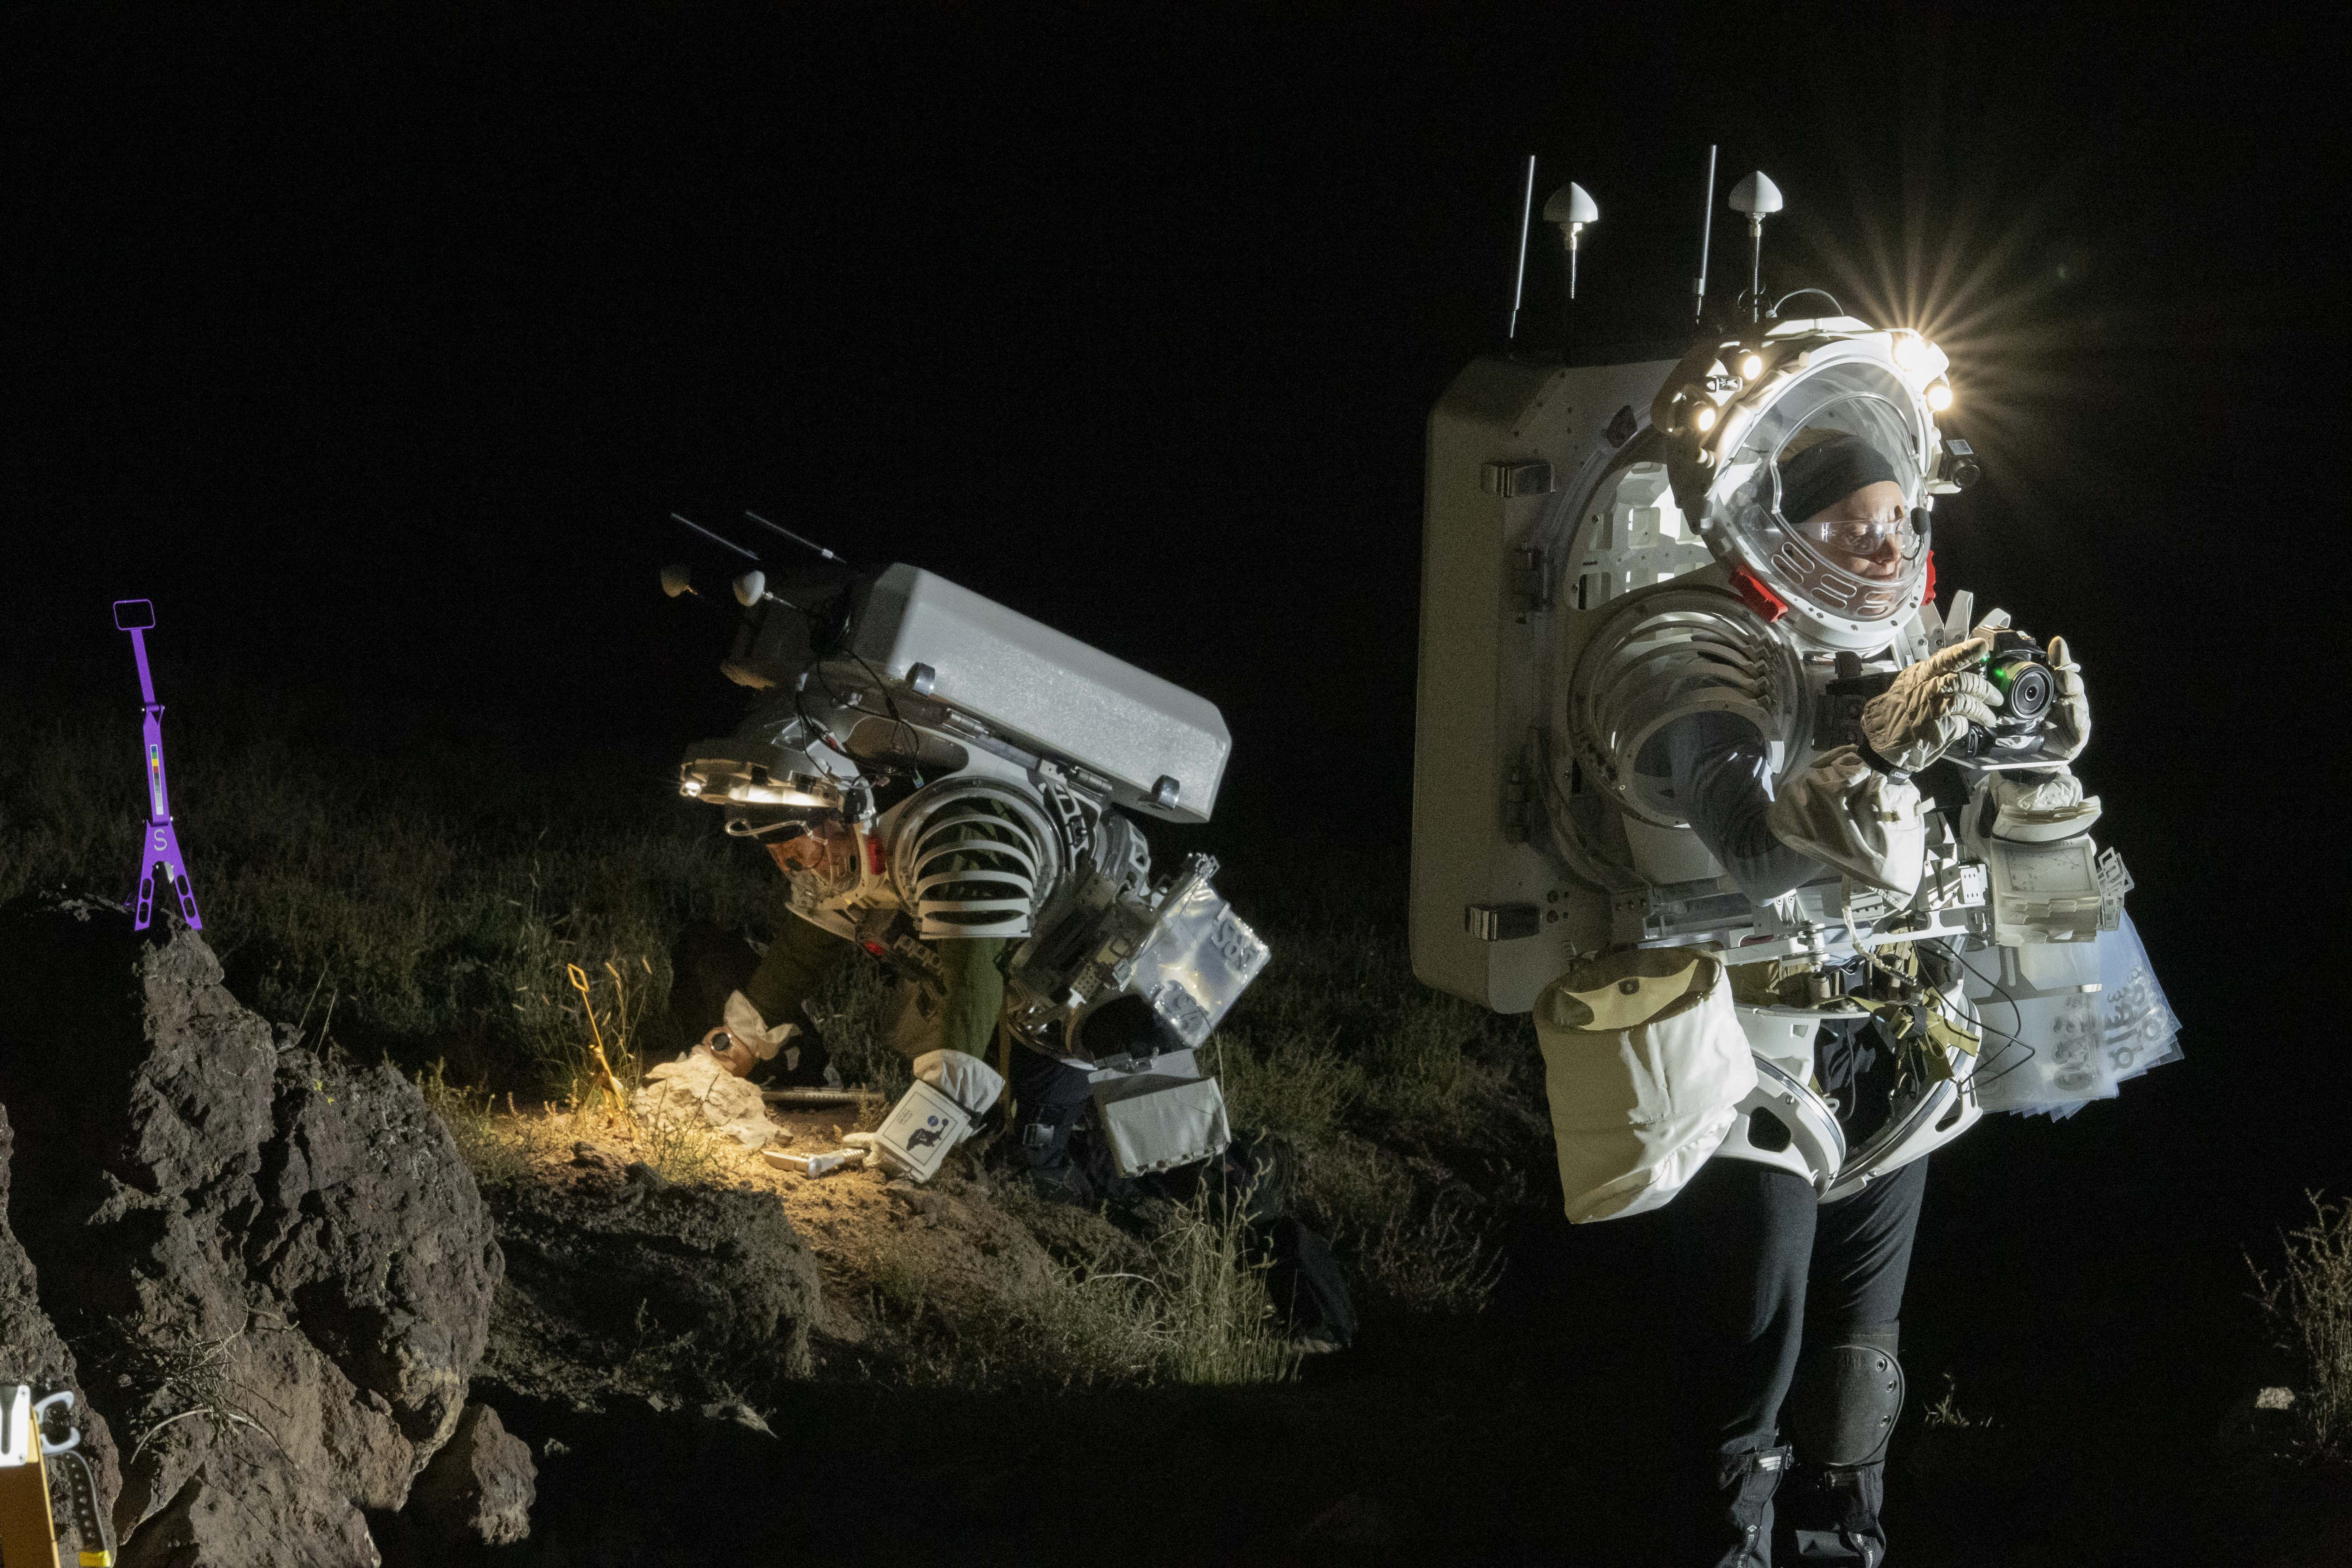
\includegraphics[width=0.75\textwidth]{wjs_2270_orig.jpg}
    \caption{NASA's Image of the Day for February 15th, 2023}  % Add appropriate captions for your figures!
    \label{fig:NASAIOTD}  % set this for referring to it in the text (see below)
\end{figure}

% What we did with the figure above is switch from normal text to a figure environment - once we tell LaTeX what it is, it knows that a figure is a float and you can assign information to it for cross-referencing

Figure \ref{fig:NASAIOTD} shows an EVA test in Arizona.

\subsection{Tables}
You can also add tables with a begin command, but they also have a tabular environment:  % table and tabular environments below

\begin{table}[h]
    \centering
    \begin{tabular}{|c|c|} % add | for vertical lines and hline for horizontal
        A & B \\  % double backslash is for a new line
        C & D \\ \hline
    \end{tabular}
    \caption{Caption}
    \label{tab:test}
\end{table}

Added extra vertical and horizontal lines to Table \ref{tab:test}. % lots of options for tables, including over multiple pages, horizontal, etc.

\subsection{Equations} % Lots and lots of ways to do equations, only two covered below - LaTeX was designed for math!
Equations can be added with dollar signs bracketing the text like this $E = mc^2$.

You can also do a numbered equation like with figures and tables:

\begin{equation}
    f(r,\phi) = \iint dr d\phi
    \label{eq:doubleint}  % can add cross references for equations too
\end{equation}

Equation \ref{eq:doubleint} is a demo of a double integral.


\section{Citations}
There are a few different ways to setup citations in \LaTeX, but we will not be going into all those today and just give you the basics with built-in BibTeX.

% Create .bib file in upper left, go to Google Scholar and find any reference, click on quotes below reference and then BibTeX, copy text to .bib file to use here

Here's the reference I found in Google Scholar \cite{haws2022space}.  % Basic command is \cite for any reference, see below for where LaTeX looks for the file with the information and how to format it


\section{Tips \& Tools}

\begin{itemize}
    \item Overleaf has lots of tutorials and help, be sure to check those out!  Plus \href{https://www.overleaf.com/edu/vtech}{VT's Overleaf page} has templates and other info.  Also see Overleaf's \href{https://www.overleaf.com/latex/templates/a-quick-guide-to-latex/fghqpfgnxggz}{Quick Guide} and \href{https://www.overleaf.com/latex/templates/overleaf-keyboard-shortcuts/qykqfvmxdnjf}{Keyboard Shortcuts}.
    \item \href{https://tex.stackexchange.com}{StackExchange} and similar sites have lots of Q\&A (I use these all the time!)
    \item For packages and documentation, check out \href{https://ctan.org}{ctan.org} (over 6k - no way to know all and some conflict)
    \item Last you can check \href{https://virginiatech.on.worldcat.org/search?queryString=latex\%20documents&databaseList=\&clusterResults=false\&stickyFacetsChecked=true\&baseScope=sz\%3A38864\&groupVariantRecords=false\&scope=sz\%3A38864}{our library} for \LaTeX{} books - there have been lots published, including ones for other types of documents like presentations (Beamer). % Make sure to 'escape' i.e. use \ for the %'s and &'s in URLs to avoid problems
\end{itemize}


\bibliography{mybib}  % name of the bibliography data file
\bibliographystyle{plain}  % what citation style LaTeX is using - search for documentation based on the citation package used i.e. here it is none/BibTeX (common ones are natbib and biblatex) 

\end{document}
